\documentclass{article}

% WORKING COPY (narrative revision of manuscript.tex, 2026-10-09). Same tables, figures, and numbers.
% NeurIPS style, preprint (arXiv) mode. nonatbib lets us load natbib with numeric citations.
\usepackage[preprint,nonatbib]{neurips_2023}

\usepackage[utf8]{inputenc}
\usepackage[T1]{fontenc}
\usepackage[numbers,sort&compress]{natbib}
\usepackage{amsmath,amssymb}
\usepackage{graphicx}
\usepackage{booktabs}
\usepackage{microtype}
\usepackage{xcolor}
\definecolor{linkblue}{rgb}{0.0,0.0,0.6}
\usepackage{hyperref}
\hypersetup{colorlinks=true,allcolors=linkblue}

\graphicspath{{./}}

\title{Evaluating Adaptive Region Acquisition for\\
Spatial Transcriptomics Reconstruction}

\author{%
  Ayush Deo \\
  University of Southern California \\
}

\begin{document}
\maketitle

\begin{abstract}
Region-based spatial transcriptomics measures only part of a tissue section, and several recent methods
choose the next region to measure from the expression already measured. Whether this adaptivity helps
depends on the goal. Reconstructing expression across the whole section and capturing regions of high
molecular heterogeneity (ROI detection) reward different choices, and sensor-placement theory predicts
little benefit for the first. We tested both goals in a retrospective simulator built from 22 human HEST-1k
slides (7 Visium HD, 15 Visium; 18 studies; four tissues). Image encoder and imputer were held fixed, and
adaptive policies were compared with strong non-adaptive placement. Twenty-four primary comparisons, with
decision rules, were fixed before the run; tests resample whole studies and are Holm-adjusted. For
reconstruction, adaptive policies were worse than the best non-adaptive baseline at budgets of 0.5--2\% of
regions (mean differences $-0.128$ to $-0.040$ PCC over the top-50 genes; adjusted $p<0.001$) and close to it
at 10--20\% ($-0.002$). A policy that selects directly on measured values was worse at every budget tested
($-0.136$ to $-0.165$). For ROI detection, that policy raised recall over the best coverage baseline by
$+0.001$ to $+0.042$, but no gain remained significant after adjustment ($p\ge0.36$), and none reached
significance under batched or contiguous acquisition. In secondary and exploratory analyses, a non-adaptive
diversity sampler gained a similar amount of recall, and the gains were concentrated in the Visium HD slides.
On synthetic slides with strong ROI signal the same protocol registered an advantage of $+0.10$ recall, so it
can detect one when it exists. At these budgets and on these slides, non-adaptive placement matched or exceeded
the adaptive policies for reconstruction, and no adaptive advantage for detection was supported.
\end{abstract}

\section{Introduction}

Whole-transcriptome spatial assays are costly, and region-of-interest platforms such as GeoMx
DSP~\citep{merritt2020geomx} profile only an operator-chosen subset of a section. Regions that are not
profiled can be reconstructed afterwards, usually by predicting expression from co-registered hematoxylin and
eosin (H\&E) images~\citep{jaume2024hest,xie2023bleep}. The choice of regions therefore determines two
things: how well the rest of the section can be predicted, and whether biologically distinctive regions are
measured at all.

Recent methods make this choice sequentially. SOFisher~\citep{li2026sofisher} trains a reinforcement-learning
policy that moves fields of view toward regions enriched for a target signal, using the expression measured
so far. SCR$^2$-ST~\citep{zhu2025scr2st} uses reinforcement learning to choose sampling locations for
expression prediction, with a reward dominated by coverage of a single-cell reference manifold. S2-omics~\citep{yuan2025s2omics}
takes the opposite approach: it selects ROIs from histology before any measurement in order to capture
molecular heterogeneity, and its preprint argues that sequential designs that wait for measured expression
are hard to run in practice. These methods pursue different objectives. SOFisher and S2-omics aim to capture
particular regions; reconstruction aims to predict expression everywhere.

The distinction matters because the two objectives lead to different expectations. For reconstruction,
Gaussian-process sensor placement gives a reason to expect little from adaptivity: with a fixed kernel, the
posterior variance at each location depends on where measurements were taken but not on the values observed,
so the best adaptive and non-adaptive designs coincide~\citep{krause2008near}. For detection there is no such
argument, because the targets are defined by the values themselves. A sequential policy may help one objective
and not the other, and an evaluation that reports only one cannot tell which.

We therefore asked three questions under matched conditions, with the image encoder and imputer fixed and
strong non-adaptive placement rules as comparators:
\textbf{Q1}, does conditioning region choice on measured expression improve whole-section reconstruction?
\textbf{Q2}, does it improve the capture of molecularly heterogeneous regions?
\textbf{Q3}, does any advantage survive the batched and contiguous acquisition that real platforms impose?
Because a null result is only informative if the protocol could have detected an effect, we first ran
synthetic positive controls.

Under the pre-specified rules, the reconstruction null was retained for Q1, and a detection advantage was
not supported for Q2 or Q3. Adaptive policies were worse than or close to non-adaptive placement for
reconstruction. Their detection gains were small, did not survive correction, and were approached by a
non-adaptive design. The synthetic controls show that the protocol registers a detection advantage when the
ROI signal in measured expression is strong. The contribution is an evaluation, not a new method: a
reproducible protocol on 22 human slides from 18 studies with analyses fixed in advance, and the finding that,
at the budgets tested, no adaptive policy we evaluated had a supported advantage over strong non-adaptive
placement for either objective.

\section{Related work}

\paragraph{Predicting expression from histology.}
Expression has been predicted from H\&E by contrastive retrieval~\citep{xie2023bleep}, flow matching over
spatial neighbourhoods~\citep{huang2025stflow}, diffusion~\citep{zhu2025stem}, and autoregressive
generation~\citep{genar2025}, benchmarked on HEST-1k~\citep{jaume2024hest}. We hold the predictor fixed and
vary only which regions it receives.

\paragraph{Choosing what to measure.}
Gene-panel selectors fix a set of genes~\citep{covert2023persist,reconst2026}. Region selectors range from
one-shot image rankers~\citep{spatialfinder2026} and histology-based ROI selection for molecular
heterogeneity~\citep{yuan2025s2omics} to sequential reinforcement-learning samplers~\citep{li2026sofisher,zhu2025scr2st}.
We add Gaussian-process placement baselines and score the reconstruction and detection objectives on the
same slides.

\paragraph{Active acquisition and sensor placement.}
Active feature acquisition treats measurement as a sequential policy~\citep{yin2020afa}. Variance- and
mutual-information-greedy placement are submodular and near-optimal for reconstructing a Gaussian-process
field~\citep{krause2008near}, which makes them the natural non-adaptive comparators for Q1.

\section{Methods}
\label{sec:setup}

\subsection{Slides and acquisition unit}
We used 22 human slides from HEST-1k~\citep{jaume2024hest}: prostate (6), kidney (4), lung (6), and colon (6);
7 are Visium HD and 15 are standard Visium (Appendix~\ref{app:slides}). Selection rules were fixed before the
results were seen: human tissue, whole-transcriptome assay, at least 1{,}000 spots under tissue, source image
at most 0.6\,$\mu$m/px, one slide per specimen, and at most two slides per study. The last two rules limit
dependence between slides, and the image-resolution rule keeps the image inputs comparable. The 22 slides
come from 18 HEST studies, which we treat as the independent units in all tests.

The acquisition unit (``region'') is one native spot. Visium spots are 55\,$\mu$m in diameter on a
100\,$\mu$m pitch. The Visium HD slides, as distributed by HEST, have a median spot spacing of 128\,$\mu$m on our
slides. We used the spot directly because it is the unit at which HEST provides both expression and an image
patch, and because a fixed square grid would have pooled different numbers of spots on slides with
different pixel sizes. Coordinates were converted to microns with each slide's estimated pixel size. Slides
contain 1{,}766 to 9{,}080 regions. Each region's image input is the HEST 224\,px patch at 0.5\,$\mu$m/px
centred on the spot, embedded with frozen UNI2-h~\citep{chen2024uni}. Expression is log1p-transformed, and
genes detected in fewer than 10\% of regions are removed.

\subsection{Objectives}
A policy reveals regions up to a budget, expressed as a fraction of the slide's regions (0.5\% to 20\%), and
each revealed region exposes its measured expression. \emph{Reconstruction} (Q1): a fixed imputer predicts
the unprofiled regions from the profiled ones, and we score the per-gene Pearson correlation over unprofiled
regions, averaged over the top-50 highly variable genes (PCC), the HEST-Benchmark target~\citep{jaume2024hest}.
\emph{ROI detection} (Q2): following the heterogeneity objective of S2-omics~\citep{yuan2025s2omics}, ROIs are
the 20\% of regions with the highest local molecular heterogeneity, defined as the variance of top-50-gene
expression across a region's 8 nearest spatial neighbours, averaged over genes; we score recall, the fraction
of ROI regions that were profiled. ROIs and gene sets come from ground truth and are used only for scoring.

\subsection{Imputer}
The primary imputer (graphflow) maps image principal components through 512 random Fourier features, fits a
ridge regression to the profiled regions' expression, and then runs 20 steps of message passing on a fixed
8-nearest-neighbour graph in image-and-space features, holding profiled regions at their measured values.
We used one fixed imputer for every policy so that differences between policies reflect selection alone. One
property of this imputer governs how the policies should be read: its \emph{predictions} depend on the
measured values, but its \emph{uncertainty}, one minus the graph influence reaching a region from profiled
nodes, depends only on which regions are profiled. A $k$-nearest-neighbour and a regression-kriging imputer
were run on the earlier slide set only (Appendix~\ref{app:imputers}).

\subsection{Policies}
The policies fall into four groups according to what they test.
\emph{Non-adaptive designs}: random (5 seeds), farthest-point in space (grid), $k$-means on image embeddings
with medoids, a reimplementation of a one-shot image ranker~\citep{spatialfinder2026}, and variance-greedy and
mutual-information (MI)-greedy placement with an RBF kernel on joint image and coordinate
features~\citep{krause2008near}.
\emph{Sequential, value-independent}: error-reduction selects the region whose 15 nearest unprofiled
neighbours in the imputer's feature space have the largest summed imputer uncertainty, and maximum-uncertainty
selects the region of highest uncertainty. Under graphflow their choices depend on the profiled set but not
on the measured values, so they are fixed designs computed sequentially.
\emph{Value-conditioned}: each candidate is scored by the standardized kernel-weighted local variance of the
measured expression around it plus 0.5 times its standardized distance to the nearest profiled region,
starting from the region nearest the slide centroid. Its choices depend on the measured values, so it is the
direct test of Q1 and Q2.
\emph{Competitor objectives}: a diversity sampler (farthest-point in joint image and space, after the
coverage-dominated reward of SCR$^2$-ST~\citep{zhu2025scr2st}; non-adaptive) and an ROI-seeking sampler (moves
toward measured regions whose expression deviates most from the measured mean, after
SOFisher~\citep{li2026sofisher}; adaptive). These reimplement the stated objectives inside our simulator and
are not the authors' trained models.

\subsection{Positive controls}
To check that a null result would not simply reflect an insensitive protocol, we generated synthetic
$20\times20$ slides with image-unpredictable, spatially clustered structure (8 slides per setting, 10\% budget,
$k$-NN imputer). For reconstruction we varied the correlation length of the hidden structure and added a
non-deployable \emph{difficulty oracle} that orders regions by true local heterogeneity weighted by distance to
regions already chosen. It uses ground truth but is a heuristic, not a proven upper bound. For detection we
varied the amplitude $\alpha$ with which the ROIs appear in measured expression. These controls use slide-level
bootstrap intervals over the 8 synthetic slides and are descriptive.

\subsection{Comparators and statistical analysis}
For reconstruction, a policy's comparator on each slide is the best of the five non-adaptive policies other
than random (``best non-adaptive''); for detection and Q3 it is the best of $k$-means, grid, and MI-greedy
(``best coverage''). Taking the per-slide maximum favours the baseline, so a positive margin is conservative
evidence for adaptivity. For each margin (policy minus comparator, per slide) we report the mean, a 95\%
percentile bootstrap CI that resamples whole studies (5{,}000 resamples), and an exact two-sided sign-flip
test that flips the signs of whole studies (all $2^{18}$ patterns). Resampling studies rather than slides
accounts for slides from the same study being related.

The analysis plan was committed to the repository before the 22-slide run. Results fall into four categories,
which we keep distinct throughout.
\emph{Confirmatory}: a primary family of 24 margins: error-reduction versus best non-adaptive at six budgets;
value-conditioned versus best coverage for reconstruction and for detection at four budgets; and the
value-conditioned reconstruction and detection margins in the five acquisition settings of Q3. $P$-values in
this family are Holm-adjusted~\citep{holm1979simple} ($p_H$). The pre-specified rules were: the reconstruction
null is retained if the primary reconstruction margins are at most zero and none is significantly positive
after Holm adjustment; a detection advantage is claimed only for a positive margin with $p_H<0.05$.
\emph{Secondary}: other margins stored by the same experiments (competitor samplers, gene-set sensitivity),
Holm-adjusted within their experiment where stated.
\emph{Descriptive}: per-tissue means, the synthetic controls, the five-slide imputer comparison, and the native
SOFisher run.
\emph{Exploratory or post hoc}: the platform split, the maximum-uncertainty margin over the best non-adaptive
baseline, and the equivalence tolerance of 0.01 PCC, all defined after the results were seen.

\section{Results}

\subsection{The protocol can register an adaptivity advantage}
The synthetic controls bear on how to read the real-slide results. For reconstruction, even the difficulty
oracle stayed below the best coverage baseline at every correlation length: its margin was $-0.105$ and
$-0.066$ PCC at the two shortest lengths and between $-0.013$ and $-0.020$ at the three longer ones, with every
CI below zero (Figure~\ref{fig:controls}a). For detection, the value-conditioned margin over best coverage grew
with the ROI amplitude, from $-0.045$ at $\alpha=0$ to $+0.052$ (95\% CI $+0.033$ to $+0.071$) at $\alpha=4$ and
$+0.101$ ($+0.065$ to $+0.135$) at $\alpha=8$, and was positive on all 8 slides in both of the latter settings
(Figure~\ref{fig:controls}b). The error-reduction policy, which targets the imputer's uncertainty (under $k$-NN,
the variance of measured expression among neighbours) rather than heterogeneity, stayed at or below zero.

Two consequences follow. The simulator and recall metric can show a value-adaptivity advantage for detection,
so a null result on real slides is informative about the slides rather than only about the protocol. And in
this synthetic setting, even an ordering informed by true local difficulty did not improve reconstruction,
which anticipates the answer to Q1.

\begin{figure}[t]
\centering
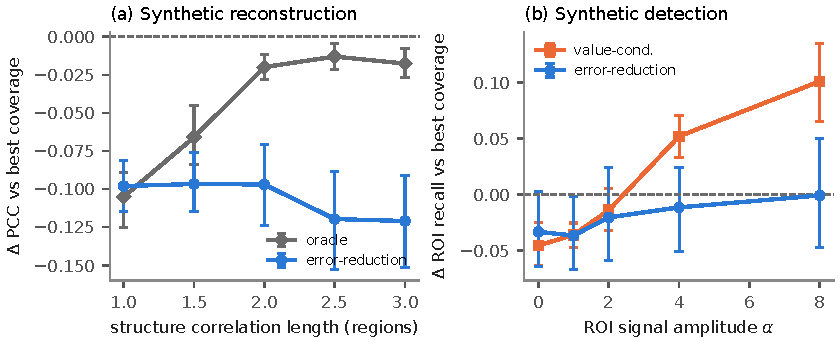
\includegraphics[width=0.85\textwidth]{fig_controls.pdf}
\caption{Synthetic controls (8 slides per point, 10\% budget, mean and 95\% bootstrap CI over slides).
(a) Reconstruction margin over the best coverage baseline versus the correlation length of the hidden
structure, for a ground-truth difficulty oracle and the error-reduction policy. (b) Detection-recall margin
versus ROI signal amplitude. The dashed line marks zero.}
\label{fig:controls}
\end{figure}

\subsection{Q1: Reconstruction}
No sequential policy improved reconstruction at any budget. Absolute accuracy is in Table~\ref{tab:recon}, and the
confirmatory margins are in Table~\ref{tab:primary} and Figure~\ref{fig:main}a. The error-reduction policy was
below the best non-adaptive baseline by 0.128, 0.083, and 0.040 PCC at 0.5\%, 1\%, and 2\% ($p_H<0.001$; lower in
all 18 studies at 0.5\% and 1\% and in 17 of 18 at 2\%) and by 0.011 at 5\% ($p_H=0.057$). At 10\% and 20\% the
margins were $-0.002$. No primary reconstruction margin was positive, so the reconstruction null is retained
under the pre-specified rule.

The imputer property noted in Methods frames this result. Under graphflow the error-reduction and
maximum-uncertainty policies are fixed designs computed one region at a time, so Q1 here compares one kind of
fixed design with others; at small budgets the uncertainty-driven designs reconstructed worse than $k$-means
or MI-greedy placement, and the gap closed as the budget grew. In a post hoc check, the 90\% study-cluster CIs at 10\% and 20\%, $[-0.006, +0.001]$ and
$[-0.003, +0.001]$, lie within $\pm0.01$ PCC, so at that tolerance (chosen after seeing the data) the
error-reduction policy and the best non-adaptive baseline are equivalent. The maximum-uncertainty policy
behaved similarly (Table~\ref{tab:recon}); in a post hoc comparison it was $+0.001$ above the best
non-adaptive baseline at 20\% (95\% CI $-0.001$ to $+0.003$, unadjusted $p=0.35$).

The value-conditioned policy, the direct test of value-adaptivity, was below best coverage at every budget, by
0.136 to 0.165 PCC ($p_H<0.001$). It reached 0.544 at 20\% (Table~\ref{tab:recon}), against 0.696 to 0.707 for
the individual coverage policies. A plausible reading, which we did not test directly, is that steering
measurements toward locally variable areas reduced the spread that reconstruction relies on.

\begin{table}[t]
\centering
\caption{Absolute reconstruction accuracy (PCC over the top-50 genes on unprofiled regions), mean over 22
slides, graphflow imputer. ``Best per slide'' is the highest-scoring non-adaptive policy on each slide.
Value-conditioned selection was run at 2--20\% only.}
\label{tab:recon}
\small
\begin{tabular}{lcccccc}
\toprule
 & \multicolumn{3}{c}{Non-adaptive} & \multicolumn{3}{c}{Adaptive} \\
\cmidrule(lr){2-4}\cmidrule(lr){5-7}
Budget & best per slide & MI-greedy & $k$-means & error-red. & max-unc. & local-var. \\
\midrule
0.5\% & 0.470 & 0.412 & 0.449 & 0.343 & 0.348 & -- \\
1\% & 0.550 & 0.522 & 0.534 & 0.467 & 0.462 & -- \\
2\% & 0.607 & 0.599 & 0.598 & 0.567 & 0.562 & 0.471 \\
5\% & 0.660 & 0.659 & 0.653 & 0.650 & 0.648 & 0.513 \\
10\% & 0.687 & 0.685 & 0.679 & 0.684 & 0.685 & 0.535 \\
20\% & 0.709 & 0.707 & 0.696 & 0.708 & 0.710 & 0.544 \\
\bottomrule
\end{tabular}
\end{table}

\begin{table}[t]
\centering
\caption{Primary (confirmatory) margins over 22 slides (18 study clusters). $\Delta$ is the mean per-slide
difference with a 95\% bootstrap CI that resamples studies; $p_H$ is the exact study-level sign-flip $p$-value,
Holm-adjusted over the 24 pre-specified primary margins (this table and Table~\ref{tab:realism}).}
\label{tab:primary}
\resizebox{\textwidth}{!}{\begin{tabular}{lcccccc}
\toprule
 & \multicolumn{4}{c}{Reconstruction (PCC, top-50 genes)} & \multicolumn{2}{c}{Detection (ROI recall)} \\
\cmidrule(lr){2-5}\cmidrule(lr){6-7}
 & \multicolumn{2}{c}{error-reduction $-$ best non-adapt.} & \multicolumn{2}{c}{value-cond. $-$ best coverage} & \multicolumn{2}{c}{value-cond. $-$ best coverage} \\
\cmidrule(lr){2-3}\cmidrule(lr){4-5}\cmidrule(lr){6-7}
Budget & $\Delta$ [95\% CI] & $p_H$ & $\Delta$ [95\% CI] & $p_H$ & $\Delta$ [95\% CI] & $p_H$ \\
\midrule
0.5\% & $-0.128$ $[-0.162, -0.096]$ & $<$0.001 & -- & -- & -- & -- \\
1\% & $-0.083$ $[-0.105, -0.064]$ & $<$0.001 & -- & -- & -- & -- \\
2\% & $-0.040$ $[-0.054, -0.027]$ & $<$0.001 & $-0.136$ $[-0.171, -0.106]$ & $<$0.001 & ${+}0.001$ $[-0.004, {+}0.006]$ & 0.723 \\
5\% & $-0.011$ $[-0.018, -0.004]$ & 0.057 & $-0.148$ $[-0.180, -0.119]$ & $<$0.001 & ${+}0.013$ $[{+}0.002, {+}0.024]$ & 0.362 \\
10\% & $-0.002$ $[-0.007, {+}0.001]$ & 0.687 & $-0.152$ $[-0.186, -0.122]$ & $<$0.001 & ${+}0.021$ $[{+}0.003, {+}0.037]$ & 0.362 \\
20\% & $-0.002$ $[-0.004, {+}0.001]$ & 0.687 & $-0.165$ $[-0.217, -0.125]$ & $<$0.001 & ${+}0.042$ $[{+}0.006, {+}0.077]$ & 0.362 \\
\bottomrule
\end{tabular}}
\end{table}

\begin{figure}[t]
\centering
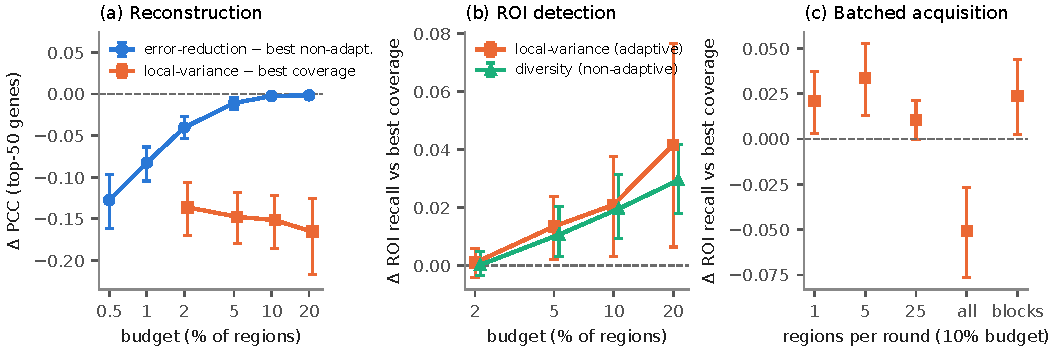
\includegraphics[width=\textwidth]{fig_main.pdf}
\caption{Margins over 22 slides, mean and 95\% CI resampling studies. (a) Reconstruction (Q1). (b) ROI-detection
recall (Q2) for the value-conditioned policy and the non-adaptive diversity sampler. (c) Detection margin of the
value-conditioned policy at 10\% budget as acquisition is batched (regions per round; ``all'' is a single
round) or made contiguous (``blocks'': each round reveals the 7 regions nearest a chosen seed) (Q3).}
\label{fig:main}
\end{figure}

\subsection{Q2: ROI detection}
The value-conditioned policy raised recall over best coverage by $+0.001$, $+0.013$, $+0.021$, and $+0.042$ at
2\%, 5\%, 10\%, and 20\% (Table~\ref{tab:primary}, Figure~\ref{fig:main}b). The unadjusted $p$-values at 5--20\%
were 0.040 to 0.044; after Holm adjustment over the primary family, all were 0.36. Under the pre-specified rule,
these margins do not establish a detection advantage. To put the estimates in scale, the coverage policies
captured ROIs at roughly the rate implied by the budget (recall 0.200--0.232 at 20\%), the value-conditioned
policy reached 0.278, and the ground-truth ordering reached 0.999 (Table~\ref{tab:detect}).

Two further analyses bear on whether the small positive estimates should be attributed to adaptivity. In the
secondary competitor analysis, the non-adaptive diversity sampler gained a similar amount over best coverage:
$+0.020$ (95\% CI $+0.009$ to $+0.031$) at 10\% and $+0.029$ ($+0.018$ to $+0.042$) at 20\%, with Holm-adjusted $p$
of 0.015 and 0.002 within that experiment, where the value-conditioned margins had adjusted $p=0.36$. This
suggests that much of the resolvable gain does not require adaptivity. In an exploratory platform split
(Appendix~\ref{app:split}), the value-conditioned detection margins at 10\% and 20\% were $+0.048$ and $+0.099$ on
the Visium HD slides (7 slides, 5 studies; with 5 clusters the smallest attainable $p$ is 0.0625) and $+0.008$
and $+0.015$ on Visium (15 slides, 13 studies; $p=0.43$ and $0.47$). The HD subset is too small to test, and we
cannot tell whether the difference reflects the platform or the particular studies.

The ROI-seeking sampler, our reimplementation of SOFisher's objective, did not improve recall ($-0.012$ to
$-0.005$, all CIs including zero) and lowered reconstruction PCC by 0.19 to 0.28. This says little about
SOFisher itself: run natively from the authors' code on its bundled mouse cortex data for 5 million steps, its
evaluation reward for captured target regions rose from a median of $-238$ early in training to $+147$ late
(descriptive; Appendix~\ref{app:sofisher}). The native method learns target capture on its own task, so the
port's result on our slides should not be read as a test of SOFisher. We could not run SCR$^2$-ST natively because its
processed training data are not publicly available.

\begin{table}[t]
\centering
\caption{Absolute ROI-detection recall (fraction of the top-20\% most heterogeneous regions profiled), mean over
22 slides. $^\dagger$Reimplementations of the stated objectives of SCR$^2$-ST (diversity, non-adaptive) and
SOFisher (ROI-seeking, adaptive) in our simulator. $^\ast$Profiles regions in order of true heterogeneity; it
uses ground truth and bounds recall from above.}
\label{tab:detect}
\small
\begin{tabular}{lccccccc}
\toprule
 & \multicolumn{3}{c}{Non-adaptive coverage} & \multicolumn{2}{c}{Competitor objectives} & & \\
\cmidrule(lr){2-4}\cmidrule(lr){5-6}
Budget & $k$-means & grid & MI-greedy & diversity$^\dagger$ & ROI-seeking$^\dagger$ & value-cond. & oracle$^\ast$ \\
\midrule
2\% & 0.018 & 0.022 & 0.018 & 0.026 & 0.021 & 0.027 & 0.100 \\
5\% & 0.050 & 0.051 & 0.046 & 0.067 & 0.050 & 0.070 & 0.250 \\
10\% & 0.110 & 0.103 & 0.094 & 0.136 & 0.104 & 0.137 & 0.500 \\
20\% & 0.232 & 0.204 & 0.200 & 0.266 & 0.232 & 0.278 & 0.999 \\
\bottomrule
\end{tabular}
\end{table}

\subsection{Q3: Batched and contiguous acquisition}
Q2 assumed that a policy sees each measurement before choosing the next region, which real platforms do not
allow. At 10\% budget we therefore revealed regions in rounds of 1, 5, or 25, or in a single round, with the
policy using only measurements available at the start of each round, and separately in contiguous blocks of 7
regions around a policy-chosen seed (Table~\ref{tab:realism}, Figure~\ref{fig:main}c). Reconstruction margins
were negative in every setting ($p_H<0.001$). Detection margins were $+0.021$, $+0.034$, and $+0.011$ for rounds
of 1, 5, and 25 and $+0.024$ for contiguous blocks, none with $p_H<0.05$ (rounds of 5: $p_H=0.073$). With a
single round the policy has no measurements and falls back to its starting rule, taking the regions nearest
the slide centroid; this compact block captured fewer ROIs than the coverage policies ($-0.051$, $p_H=0.008$).
No acquisition setting produced a supported detection advantage, so Q3 does not change the answer to Q2.

\begin{table}[t]
\centering
\caption{Value-conditioned policy minus best coverage at 10\% budget under batched and contiguous acquisition
(22 slides; $\Delta$ with 95\% CI resampling studies; $p_H$ Holm-adjusted over the primary family).}
\label{tab:realism}
\resizebox{\textwidth}{!}{\begin{tabular}{lcccc}
\toprule
 & \multicolumn{2}{c}{Reconstruction (PCC)} & \multicolumn{2}{c}{Detection (ROI recall)} \\
\cmidrule(lr){2-3}\cmidrule(lr){4-5}
Acquisition setting & $\Delta$ [95\% CI] & $p_H$ & $\Delta$ [95\% CI] & $p_H$ \\
\midrule
Sequential (1 region per round) & $-0.152$ $[-0.186, -0.122]$ & $<$0.001 & ${+}0.021$ $[{+}0.003, {+}0.037]$ & 0.362 \\
Rounds of 5 regions & $-0.129$ $[-0.175, -0.094]$ & $<$0.001 & ${+}0.034$ $[{+}0.013, {+}0.053]$ & 0.073 \\
Rounds of 25 regions & $-0.130$ $[-0.176, -0.095]$ & $<$0.001 & ${+}0.011$ $[-0.000, {+}0.021]$ & 0.362 \\
Single round (whole budget) & $-0.236$ $[-0.288, -0.188]$ & $<$0.001 & $-0.051$ $[-0.077, -0.027]$ & 0.008 \\
Contiguous blocks of 7 regions & $-0.087$ $[-0.116, -0.063]$ & $<$0.001 & ${+}0.024$ $[{+}0.002, {+}0.044]$ & 0.362 \\
\bottomrule
\end{tabular}}
\end{table}

\subsection{Sensitivity of the Q1 and Q2 results}
\emph{Gene set} (secondary). Choosing the top-50 genes from the full slide uses information a prospective
experiment would lack. Choosing them from a random 15\% reference subset changed the value-conditioned
reconstruction margins by at most 0.003, and scoring all filtered genes gave smaller but still negative margins
($-0.033$ to $-0.079$, all CIs below zero; Appendix~\ref{app:hvg}). The Q1 result does not depend on the gene
choice.
\emph{Tissue} (descriptive). The value-conditioned reconstruction margins were negative in all four tissues at
every budget, as were the error-reduction margins at 0.5--5\%; at 10--20\% the error-reduction margin in kidney
was $+0.001$ and $+0.000$. The detection margins were positive in kidney, lung, and colon and between $-0.006$
and $-0.001$ in prostate at 2--10\% (Appendix~\ref{app:split}).

\section{Discussion}

\paragraph{What the results allow us to conclude.}
For reconstruction, the evidence supports a specific statement. On these slides and at these budgets, no
policy we tested reconstructed better than the best non-adaptive design, and the policy that used measured
values most directly reconstructed worst. This agrees with the sensor-placement argument but does not test it.
Our sequential policies under graphflow were value-independent by construction, and the value-conditioned
policy optimized a different quantity (local variance) rather than the posterior error. The positive control
adds that even an ordering informed by true local difficulty did not help. Together these observations suggest
that, for whole-section reconstruction at these budgets, spreading measurements evenly mattered more than
steering them by what had been measured.

For detection, the results are weaker in both directions. The synthetic control shows that value-adaptivity can
improve detection when ROIs announce themselves strongly in measured expression. On the real slides, the
estimated gain was at most 0.042 recall at 20\% budget, against a gap of about 0.72 to the ground-truth
ordering. It did not survive correction, did not appear under any realistic acquisition setting, and was
approached by a non-adaptive diversity design. We therefore cannot rule out a small detection benefit, but we
found no evidence that adaptivity, as opposed to a better spread of measurements, produced one.

\paragraph{Practical implication.}
For budgets of 0.5--20\% of spots on slides like these, a placement rule computed before any measurement was a
sufficient comparator. MI-greedy or $k$-means placement was as accurate for reconstruction as any adaptive
policy we tested, and a non-adaptive diversity design reached recall within 0.012 of the value-conditioned policy
(0.266 against 0.278 at 20\% budget) without waiting for measurements between rounds. These results suggest
that adaptive acquisition methods be compared with such baselines, on the objective they are meant to serve.

\paragraph{Limitations.}
The simulator is retrospective: a revealed region returns its measured expression without added noise, batch
effects, or turnaround time, conditions that, if anything, favour adaptive policies. The acquisition unit is a
spot or HD pseudo-spot, which may be smaller than the ROIs used on platforms such as GeoMx, and the HD and
Visium units differ in spacing.
The 22-slide results use one imputer; the $k$-NN and kriging comparisons rest on 5 slides. The ROI definition is
one of several reasonable choices, and ROIs from expert annotation could behave differently. The competitor
samplers were evaluated as reimplementations of their objectives, not as the authors' trained systems; SOFisher
was run natively only on its own data, and SCR$^2$-ST not at all. The equivalence tolerance and the platform
split were chosen after the results were seen. Budgets above 20\% were not tested.

\section{Conclusion}

Q1: across 22 human slides from 18 studies, conditioning region choice on measured expression did not improve
whole-section reconstruction. Adaptive policies were worse than the best non-adaptive placement at 0.5--2\%
budgets, within 0.01 PCC of it at 10--20\% (post hoc tolerance), and the value-conditioned policy was worse at
every budget tested. Q2: a detection advantage was not supported; recall gains of up to 0.042 did not survive
correction for 24 comparisons, and a non-adaptive diversity sampler gained a similar amount. Q3: no batched or
contiguous acquisition setting produced a supported detection advantage. The synthetic controls show that the
protocol can register a detection advantage when ROI signal in measured expression is strong, so these nulls
describe the tested slides and budgets rather than an insensitive test. In practice, at these scales,
non-adaptive placement matched or exceeded the adaptive policies we evaluated for reconstruction, and none of
those policies had a supported detection advantage over it.

\paragraph{Reproducibility.}
Code, configuration, result files, the pre-registered analysis plan, and the scripts that regenerate every
table and figure (\texttt{scripts/14\_power\_summary.py}, \texttt{scripts/15\_paper\_assets.py}) are available at
\url{https://github.com/ayushdeo/STARE}.

\appendix

\section{Slides}
\label{app:slides}

Table~\ref{tab:slides} lists the slides. ``Cluster'' indexes the HEST study used as the resampling unit;
``Pitch'' is the median nearest-neighbour spacing of regions in microns.

\begin{table}[htbp]
\centering
\caption{The 22 slides (HEST-1k v1.3 metadata).}
\label{tab:slides}
\resizebox{\textwidth}{!}{\begin{tabular}{lllrrrrl}
\toprule
Tissue & HEST ID & Platform & Spots & $\mu$m/px & Pitch ($\mu$m) & Cluster & Study (HEST dataset title) \\
\midrule
prostate & TENX174 & Visium HD & 2385 & 0.274 & 128 & 1 & Visium HD Spatial Gene Expression Library, Human Prostate ... \\
prostate & TENX40 & Visium & 4371 & 0.345 & 100 & 2 & Human Prostate Cancer, Adenocarcinoma with Invasive Carcin... \\
prostate & MEND160 & Visium & 4079 & 0.573 & 100 & 3 & Spatially resolved clonal copy number alterations in benig... \\
prostate & TENX46 & Visium & 3043 & 0.344 & 100 & 4 & Human Prostate Cancer, Acinar Cell Carcinoma (FFPE) \\
prostate & TENX41 & Visium & 2543 & 0.345 & 100 & 5 & Normal Human Prostate (FFPE) \\
prostate & MEND144 & Visium & 4074 & 0.341 & 100 & 3 & Spatially resolved clonal copy number alterations in benig... \\
kidney & TENX173 & Visium HD & 2684 & 0.274 & 128 & 6 & Visium HD Spatial Gene Expression Library, Human Kidney (F... \\
kidney & TENX71 & Visium & 5936 & 0.274 & 100 & 7 & Human Kidney, 11 mm Capture Area (FFPE) \\
kidney & INT21 & Visium & 4975 & 0.457 & 100 & 8 & Tertiary lymphoid structures generate and propagate anti-t... \\
kidney & INT19 & Visium & 4948 & 0.457 & 100 & 8 & Tertiary lymphoid structures generate and propagate anti-t... \\
lung & TENX171 & Visium HD & 1766 & 0.274 & 128 & 9 & Visium HD Spatial Gene Expression Libraries, Post-Xenium, ... \\
lung & TENX170 & Visium HD & 1877 & 0.274 & 128 & 9 & Visium HD Spatial Gene Expression Libraries, Post-Xenium, ... \\
lung & TENX163 & Visium HD & 2487 & 0.274 & 128 & 10 & Visium HD Spatial Gene Expression Library, Human Lung Canc... \\
lung & TENX72 & Visium & 6195 & 0.274 & 100 & 11 & Human Lung Cancer, 11 mm Capture Area (FFPE) \\
lung & TENX62 & Visium & 3858 & 0.273 & 100 & 12 & Human Lung Cancer (FFPE) \\
lung & MISC20 & Visium & 3316 & 0.438 & 100 & 13 & A spatially resolved atlas of the human lung characterizes... \\
colon & TENX156 & Visium HD & 2179 & 0.274 & 128 & 14 & Characterization of immune cell populations in the tumor m... \\
colon & TENX155 & Visium HD & 2281 & 0.274 & 128 & 14 & Characterization of immune cell populations in the tumor m... \\
colon & TENX70 & Visium & 9080 & 0.274 & 100 & 15 & Human Colorectal Cancer, 11 mm Capture Area (FFPE) \\
colon & TENX92 & Visium & 6518 & 0.274 & 100 & 16 & Visium CytAssist Gene Expression Libraries of Post-Xenium ... \\
colon & MISC47 & Visium & 4818 & 0.276 & 100 & 17 & COLON MAP: Colon Molecular Atlas Project \\
colon & ZEN48 & Visium & 2385 & 0.459 & 100 & 18 & Charting the Heterogeneity of Colorectal Cancer Consensus ... \\
\bottomrule
\end{tabular}}
\end{table}

\paragraph{Changes from the earlier seven-slide analysis.} An earlier version of this analysis used seven
Visium HD slides and described regions as 112\,$\mu$m squares. Two corrections apply. First, the current HEST
metadata lists two of those slides as non-human (TENX186, \emph{Mus musculus}; TENX175, mixed human and mouse);
both are excluded here. Second, the loader had assumed 0.5\,$\mu$m/px, whereas the HD images are about
0.274\,$\mu$m/px, so the regions were about 61\,$\mu$m squares containing exactly one pseudo-spot each. The
present analysis defines the unit as the spot directly. On the five retained slides, the per-slide
value-conditioned margins (reconstruction and detection, four budgets) differ between the two runs by a
median of 0.015 (maximum 0.096), from the use of true spot positions instead of grid centres; 3 of 40 change
sign, two of them smaller than 0.005 in magnitude and one detection margin moving from $-0.050$ to $+0.015$.
With seven slides the smallest attainable exact $p$-value is 0.016, so none of the earlier margins could have
survived a correction for 24 comparisons.

\section{Platform and tissue splits}
\label{app:split}

The platform split is exploratory (not in the analysis plan); the per-tissue means are descriptive.

\begin{table}[htbp]
\centering
\caption{Selected margins by platform (with unadjusted study-level sign-flip $p$) and by tissue (mean).
With 5 HD studies the smallest attainable $p$ is 0.0625.}
\label{tab:split}
\resizebox{\textwidth}{!}{\begin{tabular}{lcccccc}
\toprule
 & HD ($n$=7, 5 cl.) & Visium ($n$=15, 13 cl.) & prostate ($n$=6) & kidney ($n$=4) & lung ($n$=6) & colon ($n$=6) \\
\midrule
Recon., error-red. (1\%) & $-0.113$ (0.062) & $-0.068$ ($<$0.001) & $-0.078$ & $-0.085$ & $-0.081$ & $-0.088$ \\
Recon., value-cond. (10\%) & $-0.103$ (0.062) & $-0.174$ ($<$0.001) & $-0.115$ & $-0.171$ & $-0.141$ & $-0.185$ \\
Detect., value-cond. (10\%) & ${+}0.048$ (0.062) & ${+}0.008$ (0.426) & $-0.001$ & ${+}0.022$ & ${+}0.036$ & ${+}0.027$ \\
Detect., value-cond. (20\%) & ${+}0.099$ (0.062) & ${+}0.015$ (0.469) & ${+}0.015$ & ${+}0.024$ & ${+}0.052$ & ${+}0.070$ \\
Detect., rounds of 5 (10\%) & ${+}0.049$ (0.250) & ${+}0.026$ (0.044) & ${+}0.016$ & ${+}0.012$ & ${+}0.046$ & ${+}0.053$ \\
\bottomrule
\end{tabular}}
\end{table}

\section{Gene-set sensitivity}
\label{app:hvg}

\begin{table}[htbp]
\centering
\caption{Value-conditioned minus best coverage reconstruction margin (PCC) under three gene sets, 22 slides,
95\% CI resampling studies (secondary).}
\label{tab:hvg}
\small
\begin{tabular}{lccc}
\toprule
Budget & per-slide top-50 HVG & reference-subset top-50 HVG & all filtered genes \\
\midrule
2\% & $-0.136$ $[-0.171, -0.106]$ & $-0.134$ $[-0.168, -0.103]$ & $-0.032$ $[-0.047, -0.021]$ \\
5\% & $-0.148$ $[-0.180, -0.119]$ & $-0.148$ $[-0.182, -0.118]$ & $-0.052$ $[-0.068, -0.040]$ \\
10\% & $-0.152$ $[-0.186, -0.122]$ & $-0.153$ $[-0.189, -0.122]$ & $-0.068$ $[-0.087, -0.052]$ \\
20\% & $-0.165$ $[-0.217, -0.125]$ & $-0.166$ $[-0.217, -0.126]$ & $-0.079$ $[-0.101, -0.061]$ \\
\bottomrule
\end{tabular}
\end{table}

\section{Imputer comparison on the earlier slide set}
\label{app:imputers}

The $k$-NN and kriging imputers were run only on the earlier slide set. Table~\ref{tab:imputers} reports the
error-reduction policy minus the best non-adaptive baseline on the five human slides from that run (legacy
unit, which equals one pseudo-spot per region on these slides), with the number of slides on which the margin
was positive. With five slides these values are descriptive.

\begin{table}[htbp]
\centering
\caption{Error-reduction minus best non-adaptive (PCC), mean over 5 human Visium HD slides (positive/total).}
\label{tab:imputers}
\small
\begin{tabular}{lccc}
\toprule
Budget & kNN & kriging & graphflow \\
\midrule
0.5\% & $-0.088$ (0/5) & $-0.088$ (2/5) & $-0.082$ (0/5) \\
1\% & $-0.114$ (0/5) & $-0.138$ (1/5) & $-0.083$ (0/5) \\
2\% & $-0.091$ (0/5) & $-0.150$ (1/5) & $-0.040$ (0/5) \\
5\% & $-0.121$ (0/5) & $-0.141$ (1/5) & $-0.011$ (1/5) \\
10\% & $-0.134$ (0/5) & $-0.133$ (0/5) & $-0.000$ (2/5) \\
20\% & $-0.145$ (0/5) & $-0.126$ (0/5) & $-0.002$ (2/5) \\
\bottomrule
\end{tabular}
\end{table}

\section{Native SOFisher run}
\label{app:sofisher}

We ran SOFisher from the authors' repository on its bundled mouse cortex data for 5 million steps (seed 222),
using the repository's cortex script. The only change was the addition of checkpoint and resume support, so
that the run could continue after interruptions. Figure~\ref{fig:sofisher} shows the evaluation reward, which
counts captured target regions. Its median over the first 5\% of training was $-238$ and over the last 10\% was
$+147$ (best 514). Rare evaluation episodes have rewards near $-1.7\times10^5$, so we plot rolling medians.

\begin{figure}[htbp]
\centering
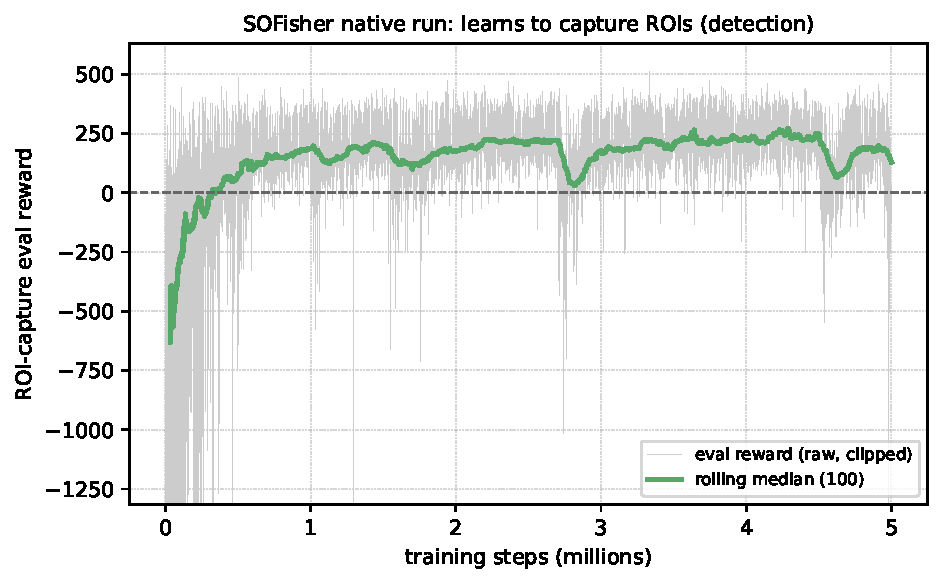
\includegraphics[width=0.7\textwidth]{fig_sofisher_native.pdf}
\caption{SOFisher evaluation reward during training (rolling median), native run.}
\label{fig:sofisher}
\end{figure}

\section{Configuration}
\label{app:repro}

All values are fixed in the released \texttt{config.py}. Seeds: global 2021; random policy $\{0,\dots,4\}$.
Imputer (graphflow): image PCA 64, random Fourier features 512 (median-heuristic bandwidth), ridge 10, graph
$k=8$, 20 steps, step size 0.5. $k$-NN imputer: $k=10$, joint image and space features. Kriging: image PCA 64,
ridge 10, residual $k=10$. Placement: feature PCA 64, median-heuristic lengthscale, noise $10^{-2}$.
Error-reduction neighbourhood 15. Value-conditioned: spatial kernel width 0.1 of the slide diagonal,
exploration weight 0.5; the ROI-seeking sampler uses the same values. Detection ROIs: top 20\% by heterogeneity
over 8 spatial neighbours. Statistics: 5{,}000 bootstrap resamples, exact sign-flip enumeration over study
clusters, Holm over 24 primary margins. The code used for the larger slides replaces dense distance computations
with sparse and incremental ones; on a 132-run check (11 policies, 3 imputers, 2 slide sizes, 2 budgets) it
reproduced the original code's selections and scores exactly.

\clearpage
\bibliographystyle{plainnat}
\bibliography{references}

\end{document}
